 % \chapter{Introduction}
\chapter{ \label{chap:Motivation}  Introduction and Motivation: \\ The Pursuit of Majorana Fermions in superconducting wires. }

\pagenumbering{arabic}
\setcounter{page}{1}

\begin{chapquote}{\textit{F. Duncan M. Haldane}}
``It started out with a toy model demonstration, and then I realized it was very good model.  You don't understand the full implications until other people start thinking it is true and they observe the big picture [...] Now, that toy model is like Hydrogen atom for topological materials- it turned out to be the first example of topological quantum matter.''
\end{chapquote}
\begin{figure}[b]
  \centering
  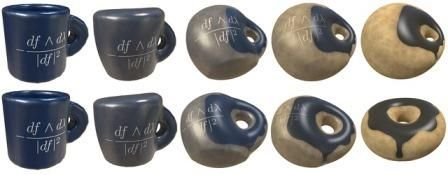
\includegraphics[scale = 0.5]{IMAGES/Majorana/Coffe&donuts.jpg}
  \caption{Up: Failed topological evolution from a cup of coffee to a sphere. Down: Smooth evolution of a coffee cup into a donut. \label{fig:Coffe}Taken from \url{https://bit.ly/2ETicqM} }
\end{figure}


In 2001, Alexei Yu Kitaev presented a toy model that could lead to the implementation of topological qubits \citep{kitaev_unpaired_2001}, an innovative idea that promised to sort out the problem of high decoherence in quantum computation. Kitaev used the properties of an exotic quasi-particle bound at the edges of a superconducting wire. This "bound state" was cataloged as a "Majorana fermion", the iconic particle predicted by Ettore Majorana in the 1930s. Majoranas were initially proposed as a real field solution of the Dirac equation, which describes fermions that are their own antiparticle\citep{wilczek_majorana_2009}.  So far, no fundamental particle with these characteristics has been observed. However, novel exciting  proposals are oriented to search these particles at the boundaries of topological superconducting wires. 



These "topological superconductors" belong to an emergent group of materials that experience phase transitions without passing through a symmetry breaking, meaning that they cannot be characterized by Landau theory. Instead, these phases of matter are described by  a new type of  order determined by topology. In mathematics, the word topology is used to describe non-local features of surfaces (or manifolds) that are preserved under smooth deformations. The clich\'e, but always educative, joke to explain this concept says that "Topologists cannot tell the difference between a donut and a coffee cup, since one of them 
can always be continuously deformed into the other through a
sequence of smooth and small alterations" (\ref{fig:Coffe}).\footnote{For decades, this has been the main reason for the absence of donuts at topology workshops.} However it wouldn't be possible to topologically transform a soccer ball into  a donut since no there is no way of putting  a hole into the ball by performing smooth deformations. We then say that coffee and donuts are topologically equivalent to each other, but not to the ball. 



The insight of topology into  the field of condensed matter physics is the following. Those materials who are attributed a topological characterization are endowed with a characteristic stability under smooth deformations (or adiabatic evolutions). Moreover, they usually present exotic excitations at its boundaries . The most famous example of this behavior is the integer quantum hall effect (IQHE), which exhibits an insulating bulk with electron currents passing through the edges of the material. More importantly, the magnetic field defines conductivity plateaus representing different topological phases. This effect is so robust that it allowed to define with high precision a resistivity standard unit $ R_K =\frac{h}{\ep^2} = 25812.807557(18) \Omega$, which had major impact in science and technology. 
% have  groundbreaking in the design of high precision devices.


Kitaev's toy model describes a one dimensional  topological chain. Similar to the IQHE, this chain exhibits bizarre edge states, which are documented as bounded Majorana quasi-particles. Besides the topological protection, these Majoranas have another important characteristic. Displayed in multi-state system Majoranas can show anionic non-abelian statistics \citep{kitaev_fault-tolerant_2003}. This means that if we have three Majorana fermions $\gamma_1 ,\gamma_2 $ and $\gamma_3$ and we, somehow, get to exchange the first two Majoranas and then the second and the third, it produces a different state than exchanging the last two Majoranas first and then the first two. This is a very interesting property for quantum computing since it allows to encode information in many body systems.  Kitaev pointed out that the combination of these two properties, topological stability and non-abelian statistics, could lead Majoranas to be the base of promising  implementation of fault-tolerant quantum computers \citep{kitaev_fault-tolerant_2001}. This marked the beginning of a new area called  topological quantum computing \cite{pachos_introduction_2012}, which combines areas as different as topology, knot theory \cite{turaev_book} and solid state physics. 

These ideas motivated the pursuit of Majorana fermions in condensed matter systems \citep{fu_superconducting_2008,sato_non-abelian_2009,alicea_new_2012,beenakker_search_2013}. Indeed, the last decade has been full of excitement, as new experiments have turned some of the theoretical predictions of the 1990s and 2000s into reality. Recently, the first evidence of Majorana bound states
in topological superconductors (TS) has been found in multiple experiments \citep{mourik_signatures_2012,das_zero-bias_2012,deng_anomalous_2012,deng_majorana_2016,zhang_quantized_2018}
following the prescription by \citet{oreg_helical_2010} and \citet{lutchyn_majorana_2010}. These experiments have been based on tunneling spectroscopy in junctions between TS and non metallic (NM) leads, where resonances have been
observed at zero energy, which is consistent with the presence of Majorana zero-energy modes. All of these facts, have contributed to the ``boom'' of Majorana wires, which has become one of the hottest research topics in Physics during the last decade. 

In this section, we will present a review of the main ideas behind the Kitaev chain (section \ref{sec:KitaevChain}) taking special attention on its topological characterization and non-abelian statistics. Finally, we will tell how that model inspired real implementations of Majorana wires in \ref{sec:exp}. This discussion will eventually bring us closer  to the main motivation of this thesis in \ref{sec:QDM}, the detection Majorana zero modes using quantum dots. 

% ----------------------------------------------------------------------



% ------------------------Section: Kitaev *------------------



\section{The Kitaev Chain \label{sec:KitaevChain}}

Kitaev's tight binding toy model  represents an spinless superconducting chain with the following Hamiltonian

\begin{equation}
H = \sum_{i=1}^N \left[ -t(a_i^{\dagger} a_{i+1} + a_{i+1}^{\dagger}a_i) -\mu a_i^{\dagger} a_{i} +  \Delta a_{i}a_{i+1} + \Delta^* a_{i+1}^{\dagger}a_i^{\dagger} \right].  \label{eq:kitaevHam}
\end{equation}



\noindent Where $\mu$ is the chemical potential, so that $\mu a_i^{\dagger} a_{i}$ is the energy associated to each step in the chain, and $t(a_i^{\dagger} a_{i+1} + a_{i+1}^{\dagger}a_i)$ represents the interaction between neighboring sites which is determined by the hopping term $t$. The remaining terms describe the superconducting properties of the system as it is established by the BCS theory of superconductivity. Here, $\Delta$ is a complex superconducting parameter with the form  $\Delta = e^{i\theta} \super$. The associated terms represent the Cooper pairs which can be created or annihilated at neighboring sites of the system hence breaking particle number. However, the system still preserves fermion parity, a property that will be very important during the rest of the project. 

There are different ways to diagonalize this Hamiltonians. The usual method is to perform a Bogoliubov-de Gennes transformation which makes the problem equivalent to diagonalize a $2N\times2N$-matrix. However, Kitaev's brilliant solution passes through another transform. Lets define the operators $\gammaA{j}$ and $\gammaB{j}$ such that

\begin{equation}
\gammaA{j} = e^{i\theta /2}a_j+ e^{-i\theta/2 } \ann_j \ \ , \ \ \gammaB{j} = -i(e^{i\theta /2}a_j - e^{-i\theta/2} \ann_j).
\label{eq:MajoranaTrans}
\end{equation}
It is simple to check that these operators are self-adjoint $(\gammaA{j}^\dagger = \gammaA{j}, \gammaA{j}^\dagger = \gammaB{j})$ , which implies that they are their own antiparticle.  Moreover, they satisfy the fermion anti-commutation relations
\begin{equation}
\begin{aligned}
\{\gammaA{i}, \gammaA{j}\} = \{ & \gammaB{i} , \gammaB{j}\} = 2\delta_{ij}  ,\\ 
  \{\gammaA{i}, \gammaB{j} & \} =0.
\end{aligned} 
\label{MajoranaRel}
\end{equation} 

\begin{figure}[t]
    \centering
    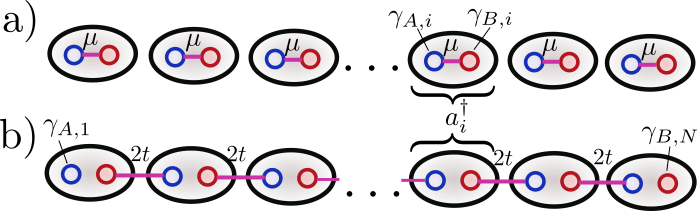
\includegraphics[scale=0.5]{IMAGES/Majorana/KitaevChain.png}
    
    \caption{ \label{fig:top.phases kitaev} Illustration of the Kitaev chain for open boundary conditions in the Majorana representation. Dirac fermions are depicted by the big globes. Each one of them contains two Majoranas (small blue and red circles) a)Represents the trivial case where the hopping and the superconducting term approaches to $0$. b) The non-trivial topological phase. The coupling is produced between Majoranas in different Dirac fermions \protect\Source{By the author} }
\end{figure} 
\noindent These relations are characteristic from a Clifford algebra, which basically describes a fermion which is its own antiparticle. A Majorana fermion. Thus, we can think $\gammaA{i} , \gammaB{i}$ as Majorana operators.

Taking the inverse of \eqref{eq:MajoranaTrans} we obtain that each  (Dirac) fermion in Hamiltonian \eqref{eq:kitaevHam} is composed by two Majorana fermions such that 
\begin{equation}
a_j = \frac{e^{-i\theta/2}}{2}(\gammaA{j}+ i\gammaB{j}) \ ,\ a^\dagger_j = \frac{e^{i\theta/2}}{2}(\gammaA{j}- i\gammaB{j}).
\end{equation}

\noindent Hence, we could adventure to say that these Majorana operators are actually splitting the Dirac fermions into real($\gammaA{}$) and imaginary $(\gammaB{})$ parts ,the same way as complex numbers are a composite of two real numbers. This is just a possible interpretation to elucidate that each Dirac fermion is composed by two types of Majorana quasi-particles just as in \ref{fig:top.phases kitaev}. 

The new Kitaev Hamiltonian in the "Majorana representation" looks like 
\begin{equation}
H = \frac{i}{2} \sum_{j=1}^N \left[ -\mu \gammaA{j}\gammaB{j}  + (t+ \super) \gammaB{j}\gammaA{j+1} + (t- \super) \gammaA{j}\gammaB{j+1} \right]+Const,\label{eq:HamMajorana}
\end{equation}

Depending on the values of parameters $\mu, t$ and $\super$ we can identify two regimes represented by the following situations:


%\begin{figure}[t]
%$$\includegraphics[scale=0.5]{KitaevtopPhases.jpg}
%\centering
%\label{top.phases kitaev}
%\caption{{\small \textit{Taken from \cite{bernevig2015topological}. Ilustration of the Kitaev chain for open boundary conditions in the Majorana representation. a)Represents the trivial case where the hopping and the superconducting term approaches to $0$. b) The non-trivial topological phase. The coupling is produced between Majoranas in different Dirac fermions }}}
%\end{figure}



\begin{figure}[t]
    \centering
    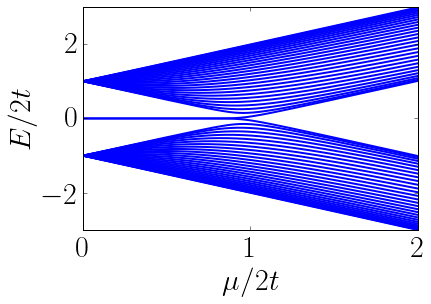
\includegraphics[scale=0.65]{IMAGES/Majorana/Spectrum.png}
    \caption{ \label{fig:KitaevSpec} Spectrum of Hamiltonian \ref{eq:HamMajorana} with $30$ sites and $t=\super$ s. Method: Numerical diagonalization. \protect \Source{By the author} }
\end{figure}


\begin{enumerate}

  \item If $\super = t = 0$ and $\mu <0$, Hamiltonian \eqref{eq:HamMajorana} becomes $\frac{-i\mu}{2} \sum_{j} \gammaA{j}\gammaB{j}$ which represents the coupling of the Majoranas in the same Dirac fermion. (See \ref{fig:top.phases kitaev} (a))

  \item If $\super = t > 0$ and $\mu =0$, the situation is much more interesting. The Hamiltonian \eqref{eq:HamMajorana} takes the form $H = 2ti\sum_{j}  \gammaB{j}\gammaA{j+1} $. This implies that the coupling is performed between  Majoranas of different Dirac fermions. Notably, this configuration leaves the edge Majorana operators ($\gammaA{1}$ and $\gammaB{N}$) uncoupled to the system (See \ref{fig:top.phases kitaev}b)). Note that these uncoupled Majorana fermions can be at any state without any  repercussion in the energy of the system. This explains the emergence of a  ground state localized at the edges of the chain. 
\end{enumerate}

These two situations are representatives of two different topological phases. The trivial phase occurs for $\frac{\mu}{2t}>1$ and the non-trivial phase appears when $\frac{\mu}{2t}<1$ (See \ref{fig:KitaevSpec}). The main characteristic of the non-trivial phase  is the creation of a robust zero-mode generated by the  uncoupled Majorana fermions at the edges of the Kitaev chain. Note that if
\begin{equation}
H = 2ti\sum_{j}  \gammaB{j}\gammaA{j+1}, \label{eq:newM} 
\end{equation}
  
\noindent it is possible to define new Dirac fermion operators as 
$$c_j = \frac{1}{\sqrt{2}} \left( \gamma_{B,j}+ i\gamma_{A,j+1} \right) \ , \ c^\dagger_j = \frac{1}{\sqrt{2}} \left( \gamma_{B,j}- i\gamma_{A,j+1} \right). $$

\noindent Then \eqref{eq:newM} becomes 
\begin{equation}
H = it\sum_{j=1}^{N-1} \left(  2c^\dagger_jc_j-1 \right). \label{eq:newM2} 
\end{equation}

Therefore, a ground state $\vert \Omega \rangle$ of this Hamiltonian is an state vacuum at all sites $j$ from $1$ to $N-1$ $(c_j\vert \Omega \rangle = 0)$. This condition allows some degeneracy since the sites at the boundary are not coupled to the Hamiltonian $\gammaA{1}$ and $\gammaB{N}$. The Dirac  operators formed by these Majoranas 
$$c_N = \frac{1}{\sqrt{2}} \left( \gamma_{B,N}+ i\gamma_{A,1} \right) \ , \ c^\dagger_N = \frac{1}{\sqrt{2}} \left( \gamma_{B,N}- i\gamma_{A,1} \right), $$ 
can be either occupied $(c^\dagger_N c_N \vert \Omega \rangle = 1)$ or empty $(c^\dagger_N c_N \vert \Omega \rangle = 0)$. Each of these results will have a different fermion parity, that is a  symmetry of our Hamiltonian.   Indeed, we can define a global parity operator as 

\begin{equation}
    \mathcal{P} =\prod_{i = 1}^N\left(  2c^\dagger_jc_j-1 \right) = \prod_{i = 1}^N -i\gamma_{B,j}\gamma_{A,j+1}= \pm 1. 
\end{equation}

In the ground state $\vert \Omega \rangle$, this parity will be  defined by the result of  $\gamma_{B,N}\gamma_{A,1}$ because the other states are fixed by $(c_j\vert \Omega \rangle = 0)$. This is an important point, since  symmetry protection is actually correlating the two opposite sites of the Kitaev chain .i.e. Any attempt to disturb one site of the chain would perturb the other site to guarantee the preservation of fermion parity.  This is a great deal,  it shows how coherent are these Majorana edge states. A possible explanation for this is the topology of the Kitaev chain, which is the objective of the next subsection.

% With these ideas in mind we are going to study the characteristics 
% of the Kitaev chain:
% \begin{itemize}
% \item Topological phase transition. \ref{subsec:top}
% \item Non-abelian statistics. \ref{subsec:non-ab}
% \end{itemize}
% These two properties are the key to implement topological quantum algorithms. 



% ---------------Subsection: Topological phase transition-------------
\subsection{Topological phase transition \label{subsec:top}}

Both regimes described previously  can be characterized with a topological parameter.  A didactic method to explain is the one used by \citeauthor{alicea_new_2012}\cite{alicea_new_2012}. First of all, suppose that we have an infinite Kitaev chain chain $(N=\infty)$ in  \eqref{eq:HamMajorana}. This system is translation invariant, hence we can make a Fourier transformation to the momentum space as

\begin{equation}
    H = 
    \sum_{k \in BZ} 
    \begin{pmatrix} 
      b_k'  & c_{k}'\\  
    \end{pmatrix}
    H_k 
    \begin{pmatrix} 
      b_{-k}'     \\ 
      c_{-k}' 
    \end{pmatrix},
    \label{PBCHam2}
\end{equation}

\noindent with the Bloch Hamiltonian equal to 

\begin{equation}
H_k = \begin{pmatrix} 
      0    &  \frac{-i \mu}{2} + it \cos k + \super  \sin k  \\ 
       \frac{i \mu}{2} - it \cos k + \super \sin k  &  0 
    \end{pmatrix}
    = (\super \sin k) \sigma_x + (\frac{\mu}{2}- t \cos k) \sigma_y.
\label{sigma}
\end{equation}




\noindent Here, $\sigma_x$ and $\sigma_y$ are the corresponding Pauli matrices. The Brilloin zone ($BZ$) is the periodic space  $[-\pi , \pi]$ which can be mapped to the unitary circle.   Equation \eqref{sigma} determines  the coordinates of the Bloch Hamiltonian in the base $\{\sigma_x, \sigma_y\}$. 

We can map these coordinates to the unitary circle by taking the norm of this vector giving
\begin{equation}
     \hat{H}_k= \frac{1}{\sqrt{\super^2 \sin^2 k + (\frac{\mu}{2}- t \cos k)^2}}
     \begin{pmatrix} 
      \super \sin k    \\ 
      \frac{\mu}{2}- t \cos k 
    \end{pmatrix}. 
\end{equation}

\noindent Note that $\super^2 \sin^2 k + (\frac{\mu}{2}- t \cos k)^2 \neq 0$ for all the values of $k$ as long as $\frac{\mu}{2t} \neq 1$ . When $\frac{\mu}{2t} = 1$, $H_{k=0}=0$, so it cannot be normalized. This is the same point were the phase transition occurs!. At any other value of $\frac{\mu}{2t}$ it is possible to normalize $H_{k}$ for all values of $k\in BZ$. The result of mapping $\hat{H}_k$ for all $k$ is a path onto the unitary circle. 

This path can take two forms as we can observe in \ref{fig:topological}. If $\frac{\mu}{2t} > 1$ the path is an arc in the upper part of the circle. In the non-trivial phase $\frac{\mu}{2t} < 1$ the path completes a wind around the circle. This is a topological difference between both phases. While the path described by the trivial phase can be contracted to a single dot, the path described by the non-trivial circle cannot be contracted. 

To determine whether the path of a given phase is type a) or type b) we only need to check if $\hat{H}_{k=0}$ and $\hat{H}_{k=\pi}$ are the same point $(0,1)$ or the opposite points $(0,1)$ and $(0,-1)$. This can be expressed into a simple equation 
\begin{equation}
    \hat{H}_{k=0,y}\hat{H}_{k=\pi,y}=\begin{cases}
1 & \mbox{trivial phase}\\
-1 & \mbox{non-trivial phase}
\end{cases},
\end{equation}
\noindent where $\hat{H}_{k=0,y}$ is the $y$-th component of $\hat{H}_{k}$. The term $\hat{H}_{k,y}$ is a particular case of the Pfaffian $\mathcal{P}(k)$, which widely used to characterize topological phase transitions involving  Majorana fermions.


\begin{figure}[t]
    \centering
    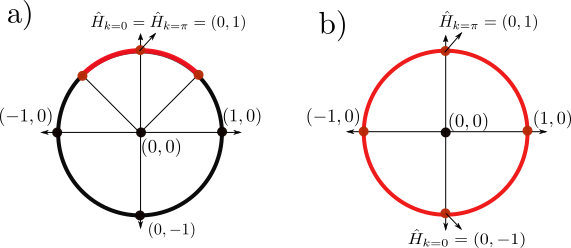
\includegraphics[scale=0.8]{IMAGES/Majorana/Topological.png}
    \caption{ \label{fig:topological}  Path of $\hat{H}_k$ for the interval $[ -\pi, \pi ]$. a) Trivial phase: The resulting path can be homotopically deformed to a point. b) Non-trivial phase: The path is a non-contractible loop around the unitary circle. \protect \Source{By the author}} 
\end{figure}


In a more general perspective, the main idea behind this topological characterization relies in the adiabatic theorem.  In simple words, the adiabatic theorem says that a slow evolution of a gaped Hamiltonian will produce a smooth evolution of its  eigenstates, so that the order of energies remains unchanged. 

A keyword in the previous definition is ``gaped''. As we can observe in  \ref{fig:KitaevSpec} the phase transition occurs at $\frac{\mu}{2t}=1$. This point is where  the gap of the Hamiltonian closes. In periodic boundary conditions no Majorana zero modes will emerge since there are no edges in the system. Therefore, the edge states with zero energy for $\frac{\mu}{2t}<1$ will not appear. We obtain that the gapless point $\frac{\mu}{2t}=1$ divides two gapped regimes. According to the adiabatic theorem, these two regions must be separated, hence meaning that no adiabatic evolution could lead from one region to the other since that would involve crossing  through a ``gapless'' Hamiltonian. 


In conclusion, these gapless Hamiltonians are forbidden in an adiabatic evolution. Hence, the banned points can be thought as "holes" in the space of Hamiltonians, which generates spaces with non-trivial topologies. Since adiabatic evolutions can be understood as smooth deformations of the Hamiltonian, the relation with topology becomes clear.  Thus, characterizing the phase transitions in the Kitaev chain, as in similar robust materials,  is mainly a topological problem, whose solution involves computing topological quantities such as Pfaffians, Chern numbers or Winding numbers, which are always integer values. 

All of these ideas lead us to an interesting question. If we have two connected topological materials, one characterized by the  number $0$ and the other by the number $1$, then what should happen at the boundary between these two discrete parameters?. Indeed some excitations are visible at the boundaries of topological materials. In the IQHE, these excitations are quantized currents passing through the edges of the placket. In the Kitaev chain  these excitations are the Majorana quasi-particles!. 

Finally,  note that in a system that preserves certain symmetries, the space of Hamiltonians has more forbidden points. Therefore, these systems have  different topological characterizations according to the protected symmetries \cite{ryu_topological_2010}.  This is the case of the Kitaev chain where the topological phase  protects the parity of the symmetry under perturbations involving the two opposed Majoranas at the edges. This endowed topological stability combined with Majorana's non-abelian statistics (next subsection) makes the Kitaev chain a promising platform for quantum computation. 




% Though this connection between physics and topology is quite interesting, I will stop here because it is taking us out of our real discussion which is Majorana fermions.  You can find more information about this in ( \Jesus{add references}). 

% -----------------------Subsection: Non-abelian Statistics -------------
\subsection{Non-abelian statistics  \label{subsec:non-ab}}


% Imagine that we have $4$ Majorana femions $\gamma_{A1}$


Imagine that we want to exchange two Majorana fermions $\gamma_1$ and $\gamma_2$ \footnote{This section is inspired on the webpage topocondmat \url{https://topocondmat.org/w2_majorana/braiding.html}, which contains an amazing tutorial about Majorana fermions and topological condensed matter. }. This procedure can be performed with an adiabatic evolution of the Hamiltonian $H(t)$ that exchanges both operators while leaving the system invariant. Therefore, after a period $T$ we require that 
\begin{equation}
\begin{aligned}
\gamma_1(T) &\rightarrow \gamma_2(0) \\
\gamma_2(T) &\rightarrow  \gamma_1(0) 
\end{aligned}
\label{eq:exchange}
\end{equation}
while  $H(0)=H(T)$. 


The adiabatic evolution is then represented by a unitary operator  $ U(t) = e^{-\frac{i}{\hbar}\int H(t)} $ and is applied according to Heisenberg's picture as 
$$\gamma_i(T) = U^\dagger(t)\gamma_iU(t).$$
 \noindent Since Majoranas preserve fermion parity,  $H$ must commute with the parity operator  $P = -i\gamma_{1}\gamma_{2} $. In a Clifford algebra generated by the operators $\gamma_1$ and $\gamma_2$ (See algebraic relations \eqref{MajoranaRel}), $$[H,\gamma_{1}\gamma_{2}]=0$$ implies that $H(t) \propto \gamma_{1}\gamma_{2}$ or $H(t)$ is a constant. Taking the non-trivial answer we obtain that the  evolution operator has the form $  U(t) = e^{\alpha(t) \gamma_1\gamma_2}$, where $\alpha(t)$ is a complex function over $t$. We can simplify this exponential noting that $\left( \gamma_1\gamma_2 \right)^2 =-1$ which after Taylor expansion reduces to
 \begin{equation}
  U(t) = \cos(\alpha(t))-\gamma_1\gamma_2\sin(\alpha(t)).
 \end{equation}

Replacing this solution in \eqref{eq:exchange} we obtain 
\begin{equation}
\begin{aligned}
\gamma_1(T) &= \gamma_1 \cos(2\alpha(T))- \gamma_2 \sin(2\alpha(T)) \rightarrow  \gamma_2\\
\gamma_2(T) &= \gamma_2 \cos(2\alpha(T))+ \gamma_1 \sin(2\alpha(T)) \rightarrow  \gamma_1,
\end{aligned}
\label{eq:nonab}
\end{equation}
which can only happen if $\alpha(T) = \pm\frac{\pi}{4}$. Hence, we conclude that the exchange operator between both Majoranas is 
\begin{equation}
U_{12} = e^{\pm\frac{\pi}{4} \gamma_1\gamma_2}=\frac{1}{\sqrt{2}}\left( 1 \pm \gamma_1 \gamma_2 \right).
\end{equation}
Note that this exchange does not depend on the  evolution, nor  the period $T$. 

\begin{figure}
  \centering
  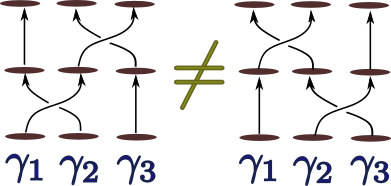
\includegraphics[scale=1]{IMAGES/Majorana/nonAb.png}
  \caption{\label{fig:Non-ab} Representation of non-abelian braiding .}
\end{figure}

% Basically if two Majorana fermions are exchange, a phase factor of $\frac{\pi}{4}$ appears. 
Now imagine that we have three Majoranas $\gamma_1, \gamma_2$ and $\gamma_3$ and we want to perform the following processes. On the first one, we exchange Majoranas $1$ and $2$ and then the Majorana in $2$ (which was initially at $1$) is exchanged with Majorana $3$ (\ref{fig:Non-ab}[Left]). On the second process, we invert the order, hence exchanging first exchange Majoranas $2$ and $3$ and then Majoranas $1$ and $2$ (\ref{fig:Non-ab}[Right]). These two cases are represented by the following operators respectively 

\begin{equation}
  \begin{aligned}
   U_{23}U_{12} = \frac{1}{2}\left( 1 + \gamma_2 \gamma_3 \right)\left( 1 + \gamma_1 \gamma_2 \right) &= \frac{1}{2}\left( 1 + \gamma_2 \gamma_3 + \gamma_1 \gamma_2 + \gamma_3 \gamma_1\right)
    \\
   U_{12}U_{23} = \frac{1}{2}\left( 1 + \gamma_1 \gamma_2 \right)\left( 1 + \gamma_2 \gamma_3 \right) &= \frac{1}{2}\left( 1 + \gamma_1 \gamma_2 +\gamma_2 \gamma_3 + \gamma_1 \gamma_3\right).
  \end{aligned}
\end{equation}
\noindent Since $\gamma_3 \gamma_1 = -\gamma_1 \gamma_3$, the outcome of both processes is essentially different, which means that it actually matters the order in which the Majoranas are exchanged .

 The particles that satisfy this strange property receive the name of non-abelian anyons. While the word "anyon" usually integrates several types of particles  including bosons and fermions, the word non-abelian makes emphasis on those anyons with non-commutative exchange statistics. 

 Non-abelian statistics is what make anyons a fantastic candidate to implement quantum algorithms. The idea of exchanging anyons can be thought as a braiding code like in \ref{fig:Non-ab}. Since the order of braiding matters, different braiding orders  can be associated to distinct algorithms. This generates another form of codifying information  which has been extendedly studied in knot theory \cite{turaev_book}. And if these anyons where topological, they will be protected from quantum decoherence \cite{nayak_non-abelian_2008}. To the date, the closest candidates to satisfy both properties (non-abelian statistics and topological characterization) are the Majorana fermions. Nonetheless, the basic braiding protocol that would unleash the keys to topological quantum computation \cite{pachos_introduction_2012} has not been measured yet. Many theoretical proposals have been set up in this direction, but there is still a long experimental road to it. 





% -------Section: Modern and Experimental-------------
% 
% 
% ---------------------------------------------------
\subsection{Real implementations of the Kitaev Chain \label{sec:exp}} 

 One of the main problems to implement real devices capable to exhibit Majorana quasi-particles at the boundaries, is that Majorana's are spin-less. Since all materials have fermion doubling,  it was necessary to endow the system with a physical property that could separate the spin energy bands. To bypass this problem, \citeauthor{lutchyn_majorana_2010}  proposed using a material with strong spin-orbit Rashba interaction \cite{manchon_new_2015} and applying a magnetic field. This would split the energy band by spin, hence destroying fermion doubling. 

This idea allowed scientists to designed the first Majorana wires. The recipe consists ingrowing a semi-conducting wire with high spin-orbit coupling, over an s'wave superconductor and inducing a Zeeman magnetic field (\ref{fig:spin-orbit}(a)). Such model is described by a Hamiltonian of the form \cite{alicea_new_2012}$(65)$

\begin{equation}
H = H_{\text{wire}} + H_\delta \label{eq:MajoranaChainHam}
\end{equation}
 with 

\begin{align}
    H_{\text{wire}} &= \sum_{\sigma \in \{\up , \dw\}} \int\mbox{d}x\ \psi^{\dagger}_\sigma(x)\left(\frac{-1}{2m}\partial_x^{2}-\mu -i\alpha\sigma_{y}\partial_x+h\sigma_{x}\right)\psi_\sigma(x),  
    \\
    H_\Delta &= \int\mbox{d} x\  \Delta\psi_{\downarrow}\psi_{\uparrow}+\Delta^{*}\psi_{\downarrow}\psi_{\uparrow}. 
\end{align}
    

\noindent Where $\psi^{\dagger}_\sigma(x)$ creates a particle at $x$ with spin $\sigma$, $\mu$ is the chemical potential, $h$ is the Zeeman splitting energy and $\alpha > 0$ is the Rashba spin-coupling parameter, favoring spin-align. The induced superconducting proximity is depicted by $H_\Delta$ where $\Delta$ is the superconducting gap. Note that this system \eqref{eq:MajoranaChainHam} has all the ingredients of the Kitaev chain. 


 If $\Delta =0$, the Bloch Hamiltonian is given by 
 \begin{equation}
 \mathcal{H}_k = \frac{k^2}{2m} -\mu + k\alpha \sigma_y +h\sigma_x.
 \end{equation}

And diagonalizing this matrix we obtain that the band splits as 
\begin{equation}
    \epsilon_\pm(k) = \frac{k^2}{2m} -\mu \pm \sqrt{(\alpha k)^2+h^2}
\end{equation}

\noindent with opposed spins as observed in the blue and red lines of \ref{fig:spin-orbit}(b).  


\begin{figure}[t]
    \centering
    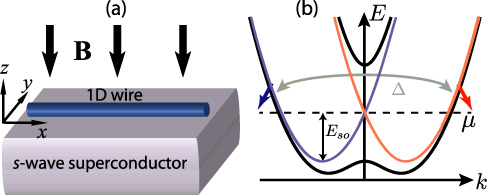
\includegraphics[scale=0.7]{IMAGES/Majorana/Mwire.png}
    \caption{ \label{fig:spin-orbit} (a) Setup of a Majorana wire with high spin-orbit coupling, over a superconducting plane and an induced Zeeman field. (b) Splitting of the energy bands with different spins in the non-superconducting regime (red and yellow bands). With superconducting proximity , a gap is opened and the red and blue energy bands are projected forming the black bands. \protect\Source{Adapted from \cite{alicea_new_2012}}}
\end{figure}


The superconducting proximity effect $(\Delta>0)$ opens a gap  that projects the upper and lower bands forming the black bands of \ref{fig:spin-orbit}(b) . This separation of both energy channels allows us to think the conduction band as an spin-less . This system enters into the topological phase  when 
\begin{equation}
  h > \sqrt{\Delta^2 +\mu^2 }. 
  \label{eq:topcond}
\end{equation}

At these points, Majorana bound states emerge at the edges of the wire.
% After these theoretical proposals different groups confirming the observation of Majorana signatures in SnSb 

This theoretical proposal led in 2012 to the first observation of Majorana signatures in InSb nanowires \footnote{A material with strong spin-orbit coupling and large $g$ factor.}, by \citeauthor{mourik_signatures_2012} from the Kavli Institute at Delft. This was a huge boost to the field which immediately attracted abundant experimental and theoretical work. 

In just 6 years, more than 5 groups have documented the observation of Majorana signatures \cite{das_zero-bias_2012,deng_anomalous_2012,nadj-perge_observation_2014,deng_majorana_2016,zhang_quantized_2018}. This signature is characterized by the emergence of a robust zero bias conductance peak ZBCP of height $\frac{2e^2}{\hbar}$ produced by the Majorana zero mode MZM localized at the edges of the wire. Though the first experiments didn't observed such an stable signature, the last year \citeauthor{zhang_quantized_2018} published a paper documenting the observation of this robust peak with the expected theoretical magnitude in and InSb wire (See \ref{fig:exp}(a)) . As can be observed in \ref{fig:exp}(b) the ZBCP increases up to $\frac{2e^2}{\hbar}$ for a strong magnetic field, where the system enters the topological phase according to equation \eqref{eq:topcond}. This zero-bias peak maintains an stable magnitude for an small range of parameters generating an small plateau, which became the first observation of a quantized Majorana signature. 



\begin{figure}[t]
\centering

     \subfloat[ \label{fig:exp1}]{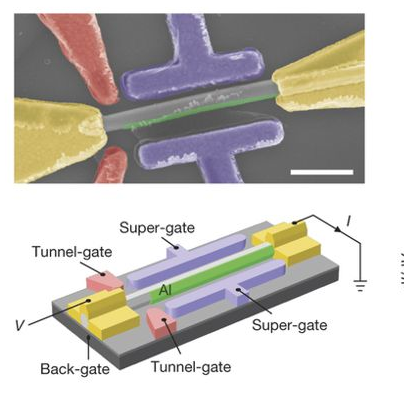
\includegraphics[scale=0.4]{IMAGES/Majorana/Exp.png}}  
     \subfloat[\label{fig:exp2}]{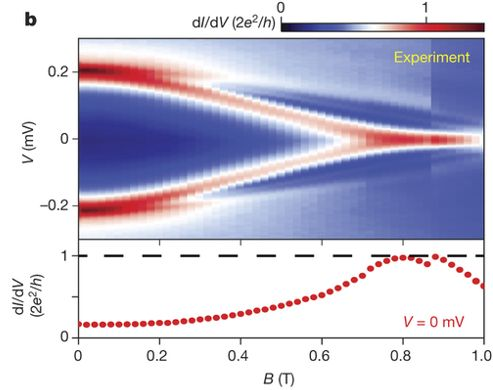
\includegraphics[scale=0.4]{IMAGES/Majorana/Exp2.png}}
\caption{ (a) Experimental setup of InSb wire exhibiting a quantized Majorana signature. (b) Up: Observed magnetic field dependence of the conductivity. Down: Zero-bias conductivity. The ZBCP rises up to the expected value $\frac{2e^2}{h}$  forming a quantized plateau at magnetic fields around $0,5T$  \label{fig:exp}\protect\Source{Adapted from \cite{zhang_quantized_2018}}}
\end{figure}

Despite the successful experimental results, there is still certain  skepticism about the existence of Majorana fermions, mainly because Majorana zero-modes (MZM) have been found in superposition with similar types of phenomena that produce zero-modes. Some examples of these are the Andreev reflection \cite{sarma_majorana_2012} or even the Kondo peak \cite{gorski_interplay_2018}. New experimental proposals focus on distinguishing MZMs from these effects and implementing  braiding protocols \cite{aasen_milestones_2016,sarma_majorana_2015,heck_coulomb-assisted_2012}. One promising idea that could lead to important results in both research lines is coupling Majorana wires with QDs. This is the objective of the following section. 


\section{\label{sec:QDM}Detecting Majorana zero modes using quantum dots}

\citeauthor{liu_detecting_2011} were the first to propose in 2011 the possibility of using QDs to detect Majorana zero modes \cite{liu_detecting_2011} . When a QD is attached to the end of a Majorana chain in the topological phase,  the Majorana Zero Mode at the end of the chain leaks inside the QD \cite{vernek_subtle_2014} producing a zero-bias conductance peak of half a quanta $\frac{e^{2}}{2h}$ through the dot. This method of detecting Majorana signatures presents important advantages:

\begin{enumerate}
  \item \textbf{It does not destroy the entire qubit information:} Other detection methods such as tunneling spectroscopy have the downside that it probes not only the end of the Topological Superconductor(TS), but its bulk as well. This completely destroys the qubit information. When attaching the Majorana chain to a QD, the conductivity is measured through the dot which does not disturb the bulk of the chain. 
  \item \textbf{Kondo-Majorana physics:} The observation of Kondo signatures in superconducting devices \cite{lee_zero-bias_2012} and the similarities between Kondo and Majorana signatures \cite{vernek_subtle_2014}  motivated  studies of prospective Kondo-Majorana physics \cite{lee_kondo_2013,gorski_interplay_2018}. 
  These two effects could co-exist at temperatures of a few mili-kelvins in quantum impurity systems.

   Quantum dots (QD) are artificial and adaptable quantum impurities, which makes them the best device to perform this kind of study. In particular, a QD-Majorana system was already studied by my advisor in a previous paper \citep{ruiz-tijerina_interaction_2015}, where he proved that it is possible separate Kondo and Majorana physics by tuning dot's gate voltage or by applying a strong magnetic field. 
  \item \textbf{Manipulation of Majorana zero modes:} Today's precise experimental experimental control over QDs makes us dream with the possibility of implementing scalable braiding proposals \ref{fig:braid}(a) and  quantum architectures for topological quantum computation \ref{fig:braid}(b). 

    These architectures perform adiabatic evolutions similar to the ones described in  \ref{subsec:non-ab} to braid Majorana fermions. This operation strongly relies on the possibility of manipulating the Majorana zero modes inside the dots. The mean idea of MZM manipulation is to  tune the gate voltage of one dot to induce the Majoranas to "move" into the other dots.  In a prospective braiding protocol, as the one described in  \cite{malciu_braiding_2018} (\ref{fig:braid}(a)), this manipulation process would have to be performed several times. However, till this moment MZM manipulation hasn't been achieved experimentally. 

\end{enumerate}

\begin{figure}[H]
  \centering
  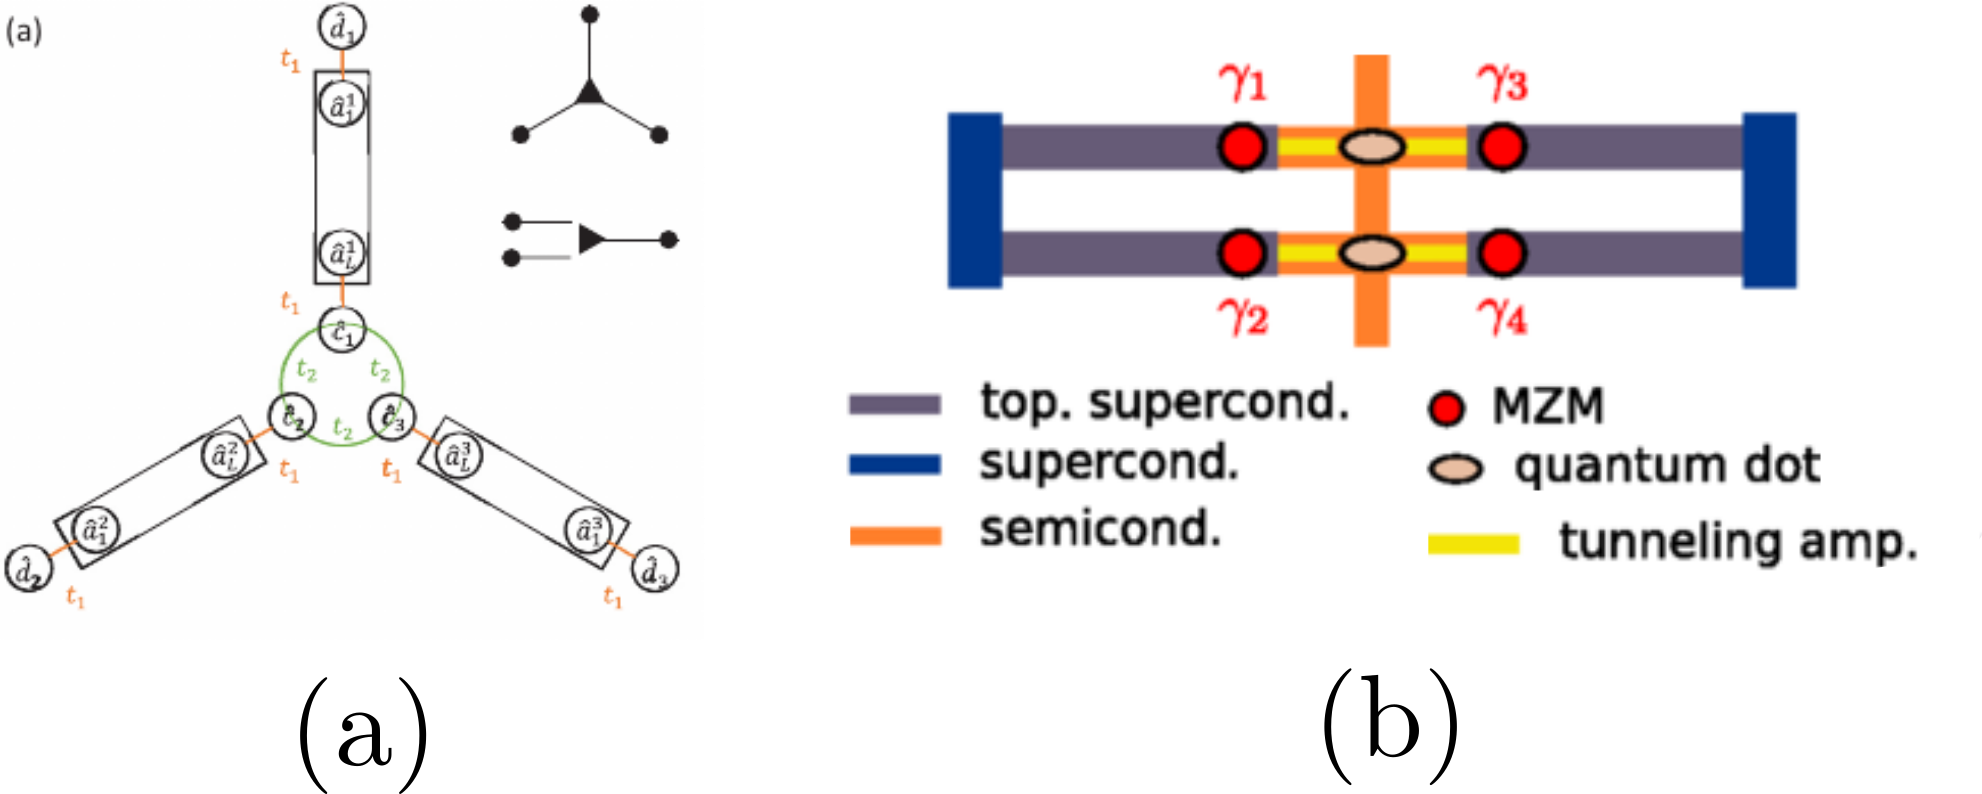
\includegraphics[scale=1]{IMAGES/Majorana/Prospective.png}
  \caption{\label{fig:braid} a) Braiding proposal b) Basic architecture with four Majorana Zero Modes in a scalable quantum computer.\protect\Source{Adapted from (a) \cite{malciu_braiding_2018} (b) \cite{karzig_scalable_2017} .}}
\end{figure}

   Nonetheless, the future for this area is still very promising. Recent experiments have documented the observation of Majorana signatures in Majorana-QD devices \cite{deng_majorana_2016,deng_nonlocality_2018} and Andreev molecules in topological superconductors attached to double quantum dots \cite{su_andreev_2017}. The next steps are clearly directed to achieve Majorana manipulation. 

   \subsection{Why double quantum dots?}

    The simplest case where Majorana manipulation is possible is in a double quantum dot (DQD). Tunneling Majorana modes in these basic structures have inspired theoretical studies \cite{silva_andreev_2016,ivanov_coherent_2017,RICCO201625} and experimental setups confirming the observations of Andreev molecules \cite{su_andreev_2017}. Even though quantum tunneling of a MZM into a double dot shows several possibilities for manipulation of MZM,  there is still no complete analysis of the transitions of the Majorana signatures between the QDs in this model.

   In this thesis we fill this gap by performing an study of the spectral density in a DQD attached to a MZM and a metallic lead. The simplicity of this model allows us to explore analytically different configurations of QD's from symmetric and linear couplings to T-junctions . We considered both non-interacting and interacting regimes, observing major agreement between both approaches about the location of the Majorana signature. While the non-interacting regime is suitable to obtain exact expressions for the Green function, the interacting case  shows how the Majorana signature co-exists with strongly correlated phenomena such as the Kondo effect  and RKKY interactions \cite{ruderman_indirect_1954,kasuya_theory_1956,yosida_magnetic_1957}. 





\section{Overview}

This thesis is integrated by $4$-major chapters:

\begin{itemize}
\item In  \ref{chap:Preliminaries}, we will take a review to the basis of quantum transport in single electron transistors, the Anderson model and the emergence of the Kondo effect in quantum dots. 

 \item In \ref{chap: Methods} we provide a description of the methods that we will use to study the Double Quantum Dot-Majorana system. To study non-interacting systems we will use the Zubarev's ballistic transport\cite{zubarev_double-time_1960} which is optimized through the Graph-Gauss-Jordan elimination algorithm define in \ref{sec:GraphMethod}. For non-interacting systems we use Wilson's Numerical Renormalization Group (NRG) technique \citep{wilson_renormalization_1975}. We will test our methods in a double quantum dot attached to a magnetic field. Hence, background information about double quantum dots systems will be presented in this chapter. 

\item In \ref{chap:Majorana} We will test our methods in the QD-Majorana system, confirming the results of previous papers \cite{dias_da_silva_transmission_2008,liu_detecting_2011} .

 % \item Majorana fermions. The discussion will start with the Kitaev chain addressing its main characteristics such as topological characterization and non-abelian statistics . Then we take a look to the real implementations of majorana chains were we will discuss the most recent experimental accomplishments  in the area.  At the end, we face the the problem of a hybrid Quantum Dot-Majorana system using the methods described in \ref{chap: Methods}.

\item The  \ref{chap:Results}  contains our major contributions to  this area. Using the methods from \ref{chap: Methods} and the previous acquired experience with the double quantum dot and the QD-Majorana model , we study in a  double quantum dot attached to a Majorana zero mode and a metallic lead. We will characterize in this simple model the transitions of the Majorana signature for distinct configurations of the dots. The final results are now part of a paper that we hope to submit for publication in the following months. 
\end{itemize}
 







